\documentclass{article}

\usepackage{defines}

\begin{document}

\tickettitle{1}{Понятие множества. Операции над множествами. {\it Билет не просмотрен Ксюшей, но проверен Артёмом}}

\define{множества}

Множество --- это совокупность или объединение некоторых предметов произвольной природы, то есть элементов этого множества.

\begin{itemize}
	\item $A, B, ...$ ---  множество
	\item $a, b, c, ...$ --- элемент множества
	\item $a$ принадлежит $A: \ a\in A$
	\item $a$ не принадлежит $A$: $a\notin A$ или $a \overline {\in}  A$
	\item $A$ --- подмножество B $\Rarr A \subset B$
	\item $A = B \Leftrightarrow  A \subset B \wedge B \subset A$
	\item $\varnothing, \Lambda$ --- пустое множество
	\item $\varnothing \in \{ \forall A\}$
\end{itemize}

\define{операции сложения}

$\exists \forall A, B:$ сумма или объединение $A$ и $B$ --- множество $C$, которое состоит из элементов, принадлежащих либо множеству $A$, либо множеству $B: C = A \cup B$

$\bigcup\limits_{\alpha} A_\alpha$ --- сумма конечного или бесконечного числа множеств.

\define{операции пересечения}

$\exists \forall A, B$:  $A \cap B$  пересечение $A$ и $B$ --- множество $C$, состоящее из элементов, которые принадлежат как множеству $A$, так и множеству $B: C = A \cap B$

$\bigcap\limits_{\alpha} A_\alpha$ --- пересечение конечного или бесконечного числа множеств.

{\bf Свойства сложения и пересечения}
\begin{enumerate}
	\item Коммутативность: $A \cup B = B \cup A$, $A \cap B = B \cap A$

	\item Ассоциативность $(A \cup B) \cup C  = A \cup (B \cup C) $, $ (A \cap B) \cap C = A \cap (B \cap C)$
\end{enumerate}
{\bf Операции сложения и пересечения связанны свойством дистрибутивности:}
\begin{align*}
	 & (A \cup B) \cap C  = (A \cap C) \cup (B \cap C) \ (1) \\
	 & (A \cap B) \cup C = (A \cup C) \cap (B \cup C) \ (2)  \\
\end{align*}
\proof \text{(1)}

\begin{enumerate}
	\item $\sqsupset x \in (A \cup B) \cap C: x \in A \cup B$ и $x \in C \Rarr x \in C$ и $(x \in A$ или $x \in B) \Rarr x \in A \cap C$ или $x \in B \cap C \Rarr x \in (A \cap C) \cup (B \cap C)$

	\item $\sqsupset x \in (A \cap C) \cup (B \cap C): x \in A \cap C$ или $x \in B \cap C \Rarr x \in C$ и $(x \in A$ или $x \in B) \Rarr x \in A \cup B$ и $x \in C \Rarr x \in (A \cup B) \cap C \qed$
\end{enumerate}

\proof \text{(2)}

Аналогично (1)

\define{операции вычитания}

$\exists \forall A, B$: разность $A$ и $B$ --- множество элементов $C$, которые принадлежат множеству $A$ и не принадлежат множеству $B: C = A \backslash B$

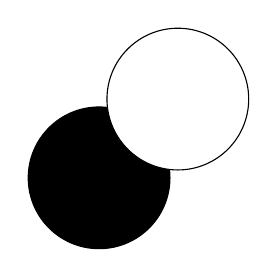
\begin{tikzpicture}
	\draw[fill=black] (0,0) circle (0.9);
	\draw[fill=white] (1,1) circle (0.9);
\end{tikzpicture}

Если $A \cap B = \varnothing \Rarr$ $A$ и $B$ --- дизъюнктные.

$A_{\triangle} B = (A \backslash B) \cup (B \backslash A) = (A \cup B) \backslash (A \cap B)$  (3)

Пусть S - основное множество, которое содержит все множества, рассматриваемые в совокупности множеств. Если $A \subset S$, то S $\backslash$ A = CA (или A').

Пусть $\exists$ \{ $A_{\alpha}$ \}, тогда имеет место следующие соотношения:
\begin{align*}
	\text{Соотношения двойственности}
	\begin{cases}
		S \backslash \bigcup\limits_{\alpha} A_\alpha = \bigcap\limits_{\alpha} (S \backslash A_{\alpha})  (4) \\
		S \backslash \bigcap\limits_{\alpha} A_\alpha = \bigcup\limits_{\alpha} (S \backslash A_{\alpha})  (5) \\
		C \bigcup\limits_{\alpha} A_\alpha = \bigcap\limits_{\alpha} C A_{\alpha}   (4')                       \\
		C \bigcap\limits_{\alpha} A_\alpha = \bigcup\limits_{\alpha} C A_{\alpha}   (5')
	\end{cases}
\end{align*}

Пусть $a \in \bigcup\limits_{\alpha} C A_{\alpha} \Rarr a \in A_{\alpha}$ при некотором номере $\alpha_{0}$

$a \in S \Rarr a \in S$ и $a \in A_{\alpha_{0}} \Rarr a \notin \bigcap\limits_{\alpha} A_{\alpha}$ и $a \in S \Rarr a \in C \bigcap\limits_{\alpha} A_{\alpha}$.

Пусть $a \in C \bigcap\limits_{\alpha} A_{\alpha} \Rarr a \in S$ и $a \notin A_{\alpha}$ при некотором $\alpha = \alpha$' $\Rarr a \notin \bigcup\limits_{\alpha} A_{\alpha}$ и $a \in S \Rarr C \bigcup\limits_{\alpha} A_{\alpha}$

\end{document}
